\documentclass[a4paper,12pt,final]{article}
% Generic commands
\usepackage{draftcommands}

% Sets margins
\usepackage[lmargin=1in,rmargin=1in,bmargin=1in,tmargin=.75in]{geometry}

% For hyperlinks, as usual
\usepackage{hyperref}

% The list of publications (with links)
\usepackage[backend=biber,maxcitenames=1,doi=true,url=true,sorting=ydnt]{biblatex}
\addbibresource{cv.bib}

% Only use url if doi is not present
\DeclareSourcemap{
  \maps[datatype=bibtex]{
    \map[overwrite]{
      \step[fieldsource=doi, final]
      \step[fieldset=url, null]
      \step[fieldset=eprint, null]
    }  
  }
}

% Multiple language

% \providecommand{\kgdlang}{english}
\providecommand{\kgdlang}{french}
\usepackage[french,english,main=\kgdlang]{babel}
\usepackage{csquotes}
\usepackage{iflang}

\def\En#1{#1}
\def\Fr#1{}
\IfLanguageName{french}{%
 \def\En#1{}\def\Fr#1{#1}
 \usepackage[T1]{fontenc}
}{}

\def\publipending{
  \En{Pending publication}%
  \Fr{Publication en cours}}

\def\publipeerreviewed{
  \En{Peer-reviewed publications}%
  \Fr{Publications peer-reviewed}}

\def\publioral{
  \En{Oral presentations}%
  \Fr{Pr\'esentations orales}}

\def\publithesis{
  \En{Thesis}%
  \Fr{Th\`ese}}


% To draw the skill circles
\usepackage{tikz}
\usetikzlibrary{calc,fadings,shadings}

\tikzfading[name=fade out,inner color=transparent!0,outer color=transparent!100]
\newcommand{\skilldisk}[1]{%
 \def\sbcolor{red}
 \hspace{.5em}%
 \def\R{.15cm}%
 \begin{tikzpicture}[remember picture]%
  \pgfmathsetmacro\A{90-3.6*#1}
  \def\bgcolor{gray!40}
  \def\fgcolor{\sbcolor!50}
  
  \fill [white] (0,0) circle (\R);
  
  \shade[ball color = \bgcolor, opacity = 0.4] (0,0) circle (\R);
  \shade[ball color = \fgcolor, opacity = 0.8] (0,\R) arc (90:\A:\R) -- (0,0) -- cycle;
 \end{tikzpicture}%
}

% Main tabular layout
% \usepackage{booktabs} % Surprisingly un-used here
\usepackage{longtable} % Pagebreak-able tables
\usepackage{makecell} % Encapsulated tabular cell contents

\usepackage{url}

% The euro symbol
\usepackage{eurosym}

% Symbols in the contact section
\usepackage{fontawesome}

 % To compute available rspace based on lspace
\usepackage{calc}

% Put pages number in footer
\usepackage{lastpage}
\usepackage{fancyhdr}

\def\fancysize{\small}

\fancyfoot[C]{\fancysize \thepage\ \En{of}\Fr{sur} \pageref*{LastPage}}
\fancyhead{}
 
\fancypagestyle{fancyfirst}{
 \fancyhead{}
 \fancyfoot[L]{\fancysize \En{Updated on} \today{}}
 \fancyfoot[C]{\fancysize \faRefresh \href{https://github.com/kgd-al/CV/raw/master/cv.pdf}{\En{Up-to date version}%
                                                                                           \Fr{Version \`a jour (Anglais)}}}
 \fancyfoot[R]{\fancysize \footnotesize Page \thepage\ \En{of}\Fr{sur} \pageref*{LastPage}}
}

\renewcommand{\headrulewidth}{0pt}
\pagestyle{fancy}
\thispagestyle{fancyfirst}

% For (excessively) pretty underlining
\usepackage{contour}
\usepackage[normalem]{ulem}
\renewcommand{\ULdepth}{2pt}
\contourlength{0.8pt}
\newcommand{\prettyuline}[1]{%
 \uline{\phantom{#1}}%
 \llap{\contour{white}{#1}}%
}

% Helper for the mail links
\def\mailto#1{\small\href{mailto:#1}{\texttt{#1}}}

% Pdf meta-data
\En{\def\me{Kevin Godin-Dubois}}
\Fr{\def\me{K\'evin Godin-Dubois}}
\makeatletter
\hypersetup{
 pdfinfo={
  Author={\me},
  Title={\me{} - CV}
 }
}
\makeatother

% No indent
\setlength\parindent{0pt}

% =============================================================================
% Draft section

% To monitor file inclusion (in git)
\listfiles 

% Overfull hbox debugging
\overfullrule=1mm

% =============================================================================
\begin{document}

% Prepare lengths
\newlength\lwidth
\setlength\lwidth{.2\textwidth}
\newlength\cwidth
\setlength\cwidth{\dimexpr2\tabcolsep}
\newlength\rwidth
\setlength\rwidth{\dimexpr\textwidth-\lwidth-\cwidth-.4pt}

% Local variables
\newlength\titlewidth
\newlength\titleoffset

% Display width repartition
% {\color{red}\rule{\lwidth}{1mm}}{\color{green}\rule{\cwidth}{1mm}}{\color{blue}\rule{\rwidth}{1mm}}

\newenvironment{sect}[2][{\\*[0pt]}]{%
 \def\title{\Large\prettyuline{\texttt{\textbf{#2}}}}%
 \setlength{\titlewidth}{\widthof{\title}}%
 \setlength{\titleoffset}{\maxof{0pt}{\lwidth-\titlewidth*\real{0.5}}}%
%  lwidth: \the\lwidth \\
%  title width: \the\titlewidth\\
%  title offset: \the\titleoffset \\
%  
 \begin{longtable}{@{}c|c@{}}%\\\\[-.75cm]
  \multicolumn{2}{l}{\hspace{\titleoffset}\title}\vspace{-2.9pt}\\*#1%\\[-10pt]
}{%
 \end{longtable}%
}%

\newcommand{\itm}[3]{%
 \makecell[t{p{\lwidth}}]{\hfill \textbf{#1} \\ \hfill #2} & \makecell[t{p{\rwidth}}]{#3} \\
}

\def\di{$\bullet$\ }
\def\dii{\hspace{1.5em} $\circ$\ }
\renewcommand{\labelitemi}{\di}
\renewcommand{\labelitemii}{\dii}

% =============================================================================
% Contents

\begin{sect}{\Huge \me}
 \itm{Contact}{}{%
  \centering\begin{tabular}[t]{c@{ }m{.35\textwidth}c@{ }m{.3\textwidth}}
   \faHome & \En{Toulouse University}
             \Fr{Toulouse I Capitole}
                                          & \faPhone & +33 5 67 06 93 91 \\
           & IRIT - CNRS UMR 5505         & \faMobile & +33 6 18 72 09 06 \\
           & 2 rue du Doyen Gabriel Marty & \faGithub & \href{https://github.com/kgd-al}{kgd-al@github.com} \\
           & 31042 Toulouse, France       & \faVimeo & \href{https://vimeo.com/godinduboisalife}{godinduboisalife} \\
%    \addlinespace[.1cm]
   \faEnvelopeO & \mailto{godindubois@gmail.com} &
     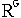
\includegraphics{misc/academicons_rgate} & \href{https://www.researchgate.net/profile/Kevin_Godin-Dubois2}{ResearchGate} \\     
  \end{tabular}
 }
 \\\\
 
 \itm{Synopsis}{}{
  {\centering\large \emph{%
    \En{A-Life Researcher on the Emergence of Cognition}%
    \Fr{Vie Artificielle et \'Emergence de la Cognition}%
  }}%
  \\\small%
  \En{After a PhD thesis focused on artificial plant-like lifeforms and their dynamics at the evolutionary scale, I plan on returning to my core interest: artificial cognition.
  More specifically, my objectives are to investigate the mechanisms by which high-level forms of interaction can be built upon low-level inputs/outputs, especially in response to environmental constraints.}
  \Fr{Suite \`a un doctorat centr\'e sur des plantes artificielles et leurs dynamiques \`a l'\'echelle \'evolutionaire, je projette de revenir \`a mon int\'er\^et principal: la cognition artificielle.
  Plus pr\'ecis\'ement, mon objectif est d'\'etudier les m\'ecanismes par lesquels des formes d'interaction de haut-niveau peuvent \^etre construites \`a travers des entr\'ees/sorties \'el\'ementaires, particuli\`erement en r\'eponse \`a des contraintes environnementales.}
 }%
 \\
 
 \itm{\En{Interests}\Fr{Int\'er\^ets}}{}{%
 \hfill
 \foreach \i/\lEn/\lFr/\c in {mew/Morphogenetic Engineering/Morphogenetic Engineering/Dubois2017,
                    phylogenetics_colored/Species Dynamics/Phylog\'enie/{GodinDubois2019b,GodinDubois2019c},
                    splinoids_combat/Artificial Cognition/Cognition Artificielle/GodinDubois2020b} {
  \begin{minipage}[t]{.2\textwidth}
   \centering
   \includegraphics[width=\textwidth]{annexes/\i} \\
   \En{\lEn}\Fr{\lFr}\cite{\c}
  \end{minipage}
  \hfill
 } 
 }
\end{sect}

\def\UnivUPS{%
  \En{Toulouse University, France}%
  \Fr{Universit\'e Paul Sabatier, France}%
}

\begin{sect}{\En{Education}\Fr{\'Education}}
 \itm{\En{PhD}\Fr{Doctorat}}{2016 - \En{July} 2020}{%
  \UnivUPS
  \\
  \En{Thesis title: \emph{``Environment-driven speciation: long term interactions in artificial plant communities''}}
  \Fr{Th\`ese: \emph{``Sp\'eciation guid\'ee par l'environnement: interactions \`a long terme de communaut\'es de plantes artificielles''}}
  \\
  {\small%
    \En{Investigated how complexification of artificial creatures could be further enhanced by moving the control apparatus around the abiotic component of an ecosystem.}%
    \Fr{\'Etude sur la mani\`ere dont le complexification de cr\'eatures artificielles pourrait \^etre am\'elior\'ee par la d\'eplacement des contr\^oleurs autour du composant abiotique d'un \'ecosyst\`eme.}
  } \\
  \textbf{Contact:} Pr. Y. Duthen (\mailto{Yves.Duthen@irit.fr})
 }
 \\
   
 \itm{Master}{2014 - 2016}{
  \UnivUPS
  \\
  {\small%
    \En{Artificial Intelligence: mathematical \& symbolic models, training methods}%
    \Fr{Intelligence Artificielle: mod\`eles math\'ematiques et symboliques, m\'ethodes d'entra\^inement}
  }
 }
 \\
 
 \itm{\En{Bachelor}\Fr{Licence}}{2011 - 2014}{
  \UnivUPS
  \\
  {\small%
    \En{Computer Science: networks, programming, systems, mathematics}%
    \Fr{Informatique: r\'eseaux, programmation, syst\`emes, math\'ematiques}
  }
 }
\end{sect}

\Fr{\newpage}

\def\teachings{\En{Teachings}\Fr{Enseignements}}
\def\internship{\En{Internship}\Fr{Stage}}
\def\months{\En{months}\Fr{mois}}
\begin{sect}{\En{Experience}\Fr{Exp\'erience}}
 \itm{\teachings}{2017 - 2019}{
  \En{Capitole University}%
  \Fr{Universit\'e Toulouse I Capitole}%
    , Toulouse, France \\
  \di L2 \En{Excel and Visual Basic for Applications}%
         \Fr{Excel et Visual Basic pour Applications}%
  \\
  \di L2 \En{Algorithms and Visual Basic}%
         \Fr{Algorithmes et Visual Basic}%
  \\
  \di L3 \En{Modeling in Database}%
         \Fr{Mod\'elisation en Base de donn\'ees}%
  \\
 }
 \\
 
 \itm{\En{Teachings}\Fr{Enseignements}}{2016 - 2017}{%
  \En{Paul Sabatier University}%
  \Fr{Universit\'e Paul Sabatier}%
    , Toulouse, France \\
  \di L2 \En{project monitoring on C programming}%
         \Fr{Encadrement de projets de programmation en C}%
  \\
 }
 \\
 
 \itm{\internship}{2016 (6 \months)}{%
  \En{Toulouse Research Institute on Computer Science (IRIT)}%
  \Fr{Institut de Recherche en Informatique de Toulouse (IRIT)}%
    , France \\%
  \emph{%
    \En{``Rule-based artificial embryogenesis in a complex 3D environment''}%
    \Fr{``Embryogen\`ese artificielle dans un environnement 3D complexe''}%
  } \\%
  {\small%
    \En{Deployed rule-based genomes on the MecaCell platform to study artificial plant growth and cell specialization.}%
    \Fr{D\'eploiement de g\'enomes \`a base de r\`egles sur la plateforme MecaCell pour \'etudier la croissance de plantes et la sp\'ecialisation cellulaire.}%
  }%
 }
 \\
 
 \itm{\internship}{2015 (3 \months)}{
  \emph{%
    \En{``Comparison of different evolutionary approaches, an application to the GECCO 2015 challenge''}%
    \Fr{``Comparaison d'approches \'evolutionnaires, une application au challenge GECCO 2015''}%
  } \\
  {\small%
    \En{Performed a performance comparison (accuracy, efficiency) between Artificial Neural and Genetic Regulatory Networks on the 2015 GECCO temperature prediction challenge data.}%
    \Fr{\'Etude sur les diff\'erences de performance entre R\'eseaux de Neurones Artificiels et R\'eseaux de R\'egulation G\'en\'etiques sur des donn\'ees de pr\'ediction de temp\'erature.}%
  } \\
  \textbf{Contact:} Pr. H. Luga (\mailto{Herve.Luga@irit.fr})
 }
 \\
 
 \itm{\internship}{2014 (2 \months)}{
  \emph{%
    \En{``Conception of an architecture for automated bird discrimination''}%
    \Fr{``Conception d'une architecture pour la discrimination d'oiseaux''}%
  } \\
  {\small%
    \En{Applied Hidden Markov Models to the BirdClef2014 challenge on the identification of specific bird species in a corpus of thousands of recordings.}%
    \Fr{Application de Mod\`eles de Markov Cach\'es au challenge BirdClef2014 pour l'identification d'esp\`eces d'oiseaux dans un corpus de plusieurs milliers d'enregistrements.}%
  } \\
  \textbf{Contact:} Pr. J. Farnias (\mailto{Jerome.Farinas@irit.fr})
 }
\end{sect}

\newcommand{\formatskill}[2]{\skilldisk{#2} \small#1}
\def\cols(#1)#2{%
 \itm{#1}{}{%
  \foreach \p/\l in {#2} {%
   \begin{minipage}{.32\rwidth}\formatskill{\l}{\p}\end{minipage}%
  }%
 }%
}
\begin{sect}{\En{Skills}\Fr{Comp\'etences}}
 \cols(\En{Programming}\Fr{\small Programmation}){%
  90/C++,
  80/{C, Java},
  70/Python}%
  
 \cols(\En{Processing}\Fr{Traitement}){%
  90/{Bash (sed, awk ...)},
  85/Gnuplot,
  70/{Octave/Matlab}
 }
 
 \cols(\En{Redaction}\Fr{R\'edaction}){%
  85/{\LaTeX /Ti\textit{k}Z},
  75/Office Software
 }
 
 \cols(\En{Systems}\Fr{Syst\`emes}){%
  85/Linux,
  70/{Windows, Android}
 }

 \cols(\En{Languages}\Fr{Langues}){%
  95/\En{French}\Fr{Fran\c cais},
  90/\En{English}\Fr{Anglais}
 }
\end{sect}
 
\begin{sect}{\En{Scholarships and Fellowships}%
             \Fr{Bourses}}
             
 \itm{2016}{70K \euro}
     {\En{PhD Fellowship from the French Minister of Higher Education and Research (MESR) - over 3 years}%
      \Fr{Bourse doctorale du Minist\`ere de l'Enseignement Sup\'erieur et de la Recherche - sur 3 ans}}
 \\
 
 \itm{2015}{10K \euro}
     {\En{Master Scholarship from the International Mathematics and Computer Science Center (LabEx CIMI, Toulouse)}%
      \Fr{Bourse de master du Centre International de Math\'ematiques et Informatique (Labex CIMI, Toulouse)}}
 \\
     
 \itm{2014}{3K6 \euro}
     {\En{Merit Scholarship from the Regional Student Welfare Office (CROUS, Toulouse) - over 2 years}%
      \Fr{Bourses de m\'erite (CROUS, Toulouse) - sur 2 ans}}
\end{sect}

\En{\newpage}

\begin{sect}[]{\En{Research Output}%
               \Fr{Production Scientifique}}
 \multicolumn{1}{m{\lwidth}}{} & \multicolumn{1}{m{\rwidth-11.6pt}}{} \\*
\end{sect}%
\vspace{-\baselineskip}
\nocite{*}%
\textbf{\publipending}
\printbibliography[heading=none, type=unpublished]
\textbf{\publipeerreviewed}
\printbibliography[heading=none, nottype=misc,nottype=unpublished]
\textbf{\publioral}
\printbibliography[heading=none, nottype=unpublished, subtype=talk]

\end{document}
